% -------------------------------------------------------------------------------------- %

\section{Numerical Methods}

\subsection{Petrov-Galerkin Methods}

The original Ritz-Galerkin method is described as follows: we are given a PDE problem in 
its \emph{weak formulation}: 
\begin{equation}
    \label{eq:weak_pde}
    \text{find } u \in \scrX \text{ such that } q(v, u) 
    = \left\langle f, v \right\rangle\ \forall\; v \in \scrW
\end{equation}
where $q$ is some elliptic sesquilinear form, $f \in \scrX$ given, 
$\left\langle \cdot, \cdot \right\rangle$ some inner product, and $\scrW$ some 
\emph{test set}. The form $q$ is typically derived from some minimization problem for a 
functional representing energy. 

The idea behind the Ritz-Galerkin method is to \emph{solve \ref{eq:weak_pde} on a 
finite-dimensional subspace:} let 
$\scrW = \spn \left\{ \psi_1, \ldots, \psi_N \right\}$ be 
$q$-linearly independent. 

Then writing 
\begin{equation}
    \label{eq:Psi}
    \Psi (x) = \left[ \psi_1 (x) \mid \ldots \mid \psi_N (x) \right] , 
\end{equation}
we make the 
approximation $u \approx \Psi c_u$ and have $v = \Psi c_v$ for $c_u, c_v \in \bbC^N$. 
Now \ref{eq:weak_pde} reduces to 
\begin{equation}
    \text{find } c_u \in \bbC^N \text{ such that } 
    q( \Psi c_v, \Psi c_u )
    = \left\langle f, \Psi c_v \right\rangle\ \forall\; c_v \in \bbC^N . 
\end{equation}
One quickly verifies that $c_u$ is the unique solution to the matrix equation $A x = b$ 
with 
\begin{equation}
    A_{i j} = q( \Psi e_i, \Psi e_j ) = q( \psi_i, \psi_j ), \quad
    b_i = \left\langle f, \Psi e_i \right\rangle 
    = \left\langle f, \psi_i \right\rangle . 
\end{equation}
where $e_i \in \bbC^N$ is the $i$-th standard unit vector. $A$ is known as the 
\emph{stiffness matrix}. 

One can extend the Ritz-Galerkin formulation by allowing the test space to differ from 
the basis space: keep $u \approx \Psi c_u$ but let 
$\scrW = \spn \left\{ \psi^*_1, \ldots, \psi^*_M \right\}$, then $A$ and $b$ become 
\begin{equation}
    A_{i j} = q( \psi^*_i, \psi_j ), \quad 
    b_i = \left\langle f, \psi^*_i \right\rangle . 
\end{equation}
In the regime $M > N$ this equation is \emph{overdetermined} so it is solved in a least 
squares sense
\begin{equation}
    \left\| A x - b \right\|_2^2 = \min_{x \in \bbC^N} !
\end{equation}
where $\left\| \cdot \right\|_2$ is the vector $\ell^2$ norm. This is known as the 
Petrov-Galerkin method. 

One can extend the method further by asking that multiple solutions for multiple right 
hand sides $(f_j)_{j=1}^N$ are computed simultaneously, that is 
\begin{equation}
    \label{eq:galerkin}
    \left\| A X - B \right\|_F^2 = \min_{X \in \bbC^{N \times N}} !, \quad 
    B_{i j} = \left\langle f_j, \psi^*_i \right\rangle 
\end{equation}
where $\left\| \cdot \right\|_F$ denotes the Frobenius norm. 

Numerically, \ref{eq:galerkin} can be solved using the Moore-Penrose inverse
\begin{equation}
    \label{eq:moore_penrose}
    X = A^\dagger B . 
\end{equation}
An exercise in matrix calculus shows that the solution can also be written in the form 
\begin{equation}
    \label{eq:adjoint_inverse}
    X = (A^* A)^{-1} A^* B . 
\end{equation}
Both forms will prove to be useful later. 


\subsection{Extended Dynamic Mode Decomposition (EDMD)}

% -------------------------------------------------------------------------------------- %

\subsubsection{The Galerkin Ansatz}

We apply the Petrov-Galerkin Ansatz to obtain a matrix approximation $K$ 
for $\left. \scrK \right|_{\scrX}$. Let 
$q(\cdot, \cdot) = \left\langle \cdot, \cdot \right\rangle$ and consider a linearly 
independent family of functions $\left\{ \psi_1, \ldots, \psi_N \right\} \subset \scrX$. 
Take delta distributions, that is $\left\langle \delta_x, \psi \right\rangle = \psi (x)$, 
for the test function(als): let $(w_i, x_i)_{i=1}^M$ represent a quadrature scheme and 
set $\psi_i^* = \sqrt{w_i} \delta_{x_i}$. 

We then solve the Galerkin equation \ref{eq:galerkin} for $f_j = \scrK \psi_j$: 
\begin{equation}
    \label{eq:edmd}
    \left\| \sqrt{W} \YX K - \sqrt{W} \YY \right\|_F^2 = \min_{K \in \bbC^{N \times N}} !
\end{equation}
with $W = \diag (w_1, \ldots, w_M)$ and 
\begin{equation}
    (\YX)_{i j} = \left\langle \delta_{x_i}, \psi_j \right\rangle = \psi_j (x_i), \quad
    (\YY)_{i j} = \left\langle \delta_{x_i}, \scrK \psi_j \right\rangle = \psi_j (\, S (x_i) \,) . 
\end{equation}

This results in the \emph{EDMD matrix} 
\begin{equation}
    \label{eq:K_edmd}
    K = \YX^\dagger \YY = (\YX^* W \YX)^{-1} (\YX^* W \YY) . 
\end{equation} 
Inverting $\YX$ involves computing the Moore-Penrose inverse of an $N \times M$ matrix, 
whereas inverting $\YX^* \YX$ involves computing the inverse of a symmetric $N \times N$ 
matrix. Depending on the relationship between $M$ and $N$ in the particular usecase, 
either formulation might be cheaper. 

Another look at the second formulation of the EDMD matrix shows that 
\begin{equation}
    \label{eq:G}
    G_{i j} \defeq 
    ( \YX^* W \YX )_{i j} 
    = \sum_{k=1}^{M} w_k \overline{\psi_i (x_k)} \psi_j (x_k)
    \xrightarrow{\makebox[1.2cm]{\scriptsize{M \to \infty}}} 
    \left\langle \psi_i, \psi_j \right\rangle_{L^2} 
    \eqdef \bbG_{i j} , 
\end{equation}
\begin{equation}
    \label{eq:A}
    A_{i j} \defeq
    ( \YX^* W \YY )_{i j} = \sum_{k=1}^{M} w_k \overline{\psi_i (x_k)} \psi_j (\, S(x_k) \,)
    \xrightarrow{\makebox[1.2cm]{\scriptsize{M \to \infty}}} 
    \left\langle \psi_i, \scrK \psi_j \right\rangle_{L^2}
    \eqdef \bbA_{i j} , 
\end{equation}
$G$ and $A$ can be computed with constant memory requirement. 

% -------------------------------------------------------------------------------------- %

\subsubsection{Functional Minimization}\label{sec:functional_minimization}

We could have arrived at equation \ref{eq:edmd} completely differently: 
keeping the test space the same as the basis space i.e. $\psi_i^* = \psi_i$. Then the 
Galerkin equation \ref{eq:galerkin} reads
\begin{equation}
    \label{eq:edmd_infinite_data}
    \left\| \bbG K - \bbA \right\|_F^2 = \min_{K in \bbC^{N \times N}} !
\end{equation}
The question is well-posed in the sense that $\left\{ \psi_1, \ldots, \psi_N \right\}$ 
is linearly independent and hence $\bbG$ is invertible. Thus,
\begin{equation}
    K = \bbG^{-1} \bbA . 
\end{equation}
We see that the EDMD matrix $K = G^{-1} A$ is a quadrature approximation of the "infinite 
data" EDMD matrix $K = \bbG^{-1} \bbA$. The benefit of this viewpoint is that it is 
\emph{ambivalent} to the inner product: as long as an one has an approximation scheme for 
$\left\langle \psi_i, \psi_j \right\rangle_\scrX$ for \emph{some} inner product space 
$\scrX$, then one can approximate the stiffness matrix $\bbG$ and target matrix $\bbA$ 
with respect to $\scrX$. From this point on, $\bbG$ and $\bbA$ will be with respect to 
the arbitrary unspecified Hilbert space $\scrX$ unless otherwise stated. 

Notice that equation \ref{eq:edmd_infinite_data} can be rewritten as a functional least 
squares minimization:
\begin{equation}
    \label{eq:edmd_functional}
    \left\| \Psi K - \scrK \Psi \right\|_{\scrX^{1 \times N}}^2 
    = \min_{K \in \bbC^{N \times N}} !
\end{equation}
where $\scrK \Psi = \left[ \scrK \psi_1 \mid \ldots \mid \scrK \psi_N \right]$ 
is understood elementwise and
$\scrX^{1 \times N}$ is the space of (row) vector-valued functions with each 
component in $\scrX$
\begin{equation}
    \left\| \left[ f_1 \mid \ldots \mid f_N \right] \right\|_{\scrX^{1 \times N}}^2
    = \left\| f_1 \right\|_{\scrX}^2 + \ldots + \left\| f_N \right\|_{\scrX}^2 . 
\end{equation}

Let us investigate $\Psi : \bbC^N \to \scrX$ a bit closer. Decompose the Hilbert space 
$\scrX = \scrW \oplus \scrV$ where  
\begin{equation}
    \scrW = \spn \left\{ \psi_j \right\}_{j=1}^N, \quad \scrV = \scrW^\perp
\end{equation}
and let $\left\{ \psi_j \right\}_{j=N+1}^\infty$ be a basis of $\scrV$. 

A short calculation using the orthogonality of $\left\{ \psi_j \right\}_{j=1}^N$ and 
$\left\{ \psi_j \right\}_{j=N+1}^\infty$ shows that for $\phi \in \scrX$, 
\begin{equation}
    \left\langle \phi, \Psi c \right\rangle 
    = \sum_{j=1}^{N} \left\langle \phi, \psi_j \right\rangle c_j . 
\end{equation}
\iffalse
Let $\phi = \sum_{i=1}^{\infty} b_i \psi_i$ and observe
\begin{align}
    \left\langle \phi, \Psi c \right\rangle
    &= \sum_{i=1}^{\infty} \sum_{j=1}^{N} b_i c_j \left\langle \psi_i, \psi_j \right\rangle \\
    &= \sum_{i=1}^{N} \sum_{j=1}^{N} b_i c_j \left\langle \psi_i, \psi_j \right\rangle \\
    &= \sum_{j=1}^{N} \left\langle \sum_{i=1}^{N} b_i \psi_i, \psi_j \right\rangle c_j \\
    &= \sum_{j=1}^{N} \left\langle \sum_{i=1}^{\infty} b_i \psi_i, \psi_j \right\rangle c_j \\
    &= \sum_{j=1}^{N} \left\langle \phi, \psi_j \right\rangle c_j . 
\end{align}
\fi
Hence the adjoint quasi-matrix $\Psi^* : \scrX \to \bbC^N$ acts as 
\begin{equation}
    \label{eq:Psi_star}
    \Psi^* \phi = \begin{pmatrix}
        \left\langle \phi, \psi_1 \right\rangle \\
        \vdots \\
        \left\langle \phi, \psi_1 \right\rangle
    \end{pmatrix} . 
\end{equation}

\begin{lemma}
    For an arbitrary basis $\left\{ \psi_j \right\}_{j=1}^N$, the orthogonal projector $\Pi$ 
    onto the space spanned by the basis is 
    \begin{equation}
        \Pi = \Psi (\Psi^* \Psi)^{-1} \Psi^* . 
    \end{equation}
\end{lemma}

\begin{proof}
    The solution of a linear least squares problem $\left\| Ax - b \right\| = \min !$ is 
    the result of orthogonally projecting $b$ onto the range of $A$, that is, $A x = \Pi b$. 
    From equation \ref{eq:adjoint_inverse} we know $x = (A^* A)^{-1} A^* b$. Therefore 
    $\Pi b = A x = A (A^* A)^{-1} A^* b$. Since this holds for arbitrary $b$, the result 
    is proven. 
\end{proof}

Using equation \ref{eq:adjoint_inverse} we see that equation \ref{eq:edmd_functional} has 
the solution 
\begin{equation}
    \label{eq:functional_K}
    K = (\Psi^* \Psi)^{-1} \Psi^* (\scrK \Psi)
\end{equation}
Inserting the definitions of $\Psi$ and $\Psi^*$ yields $K = \bbG^{-1} \bbA$ exactly as 
in equation \ref{eq:edmd_infinite_data}. 

If we view the result of applying $K$ as in equation \ref{eq:functional_K} to a vector 
$c$ as an object in $\scrX$, that is, $\Psi K c$, we see that 
\begin{equation}
    \label{eq:PKP}
    \Psi K c = \Psi (\Psi^* \Psi)^{-1} \Psi^* (\scrK \Psi) c
    = \Pi \scrK \Psi c = \Pi \scrK \Pi \Psi c . 
\end{equation}
Since this holds for arbitrary $c$ we have proven that (when viewed as an operator 
on $\scrX$) $K$ encodes precisely the action of $\Pi \scrK \Pi$, the finite section of 
$\scrK$ over $\spn \left\{ \psi_j \right\}_{j=1}^N$. In this way, the Ritz-Galerkin 
method is a special case of a finite section method. 

\begin{algorithm}
    \caption{Extended Dynamic Mode Decomposition (EDMD)}
    \label{alg:edmd}
    \begin{algorithmic}[1]
        \Require Dictionary $\left\{ \psi_j \right\}_{j=1}^N$, data points and weights 
            $\left\{ (w_i, x_i) \right\}_{i=1}^M$
        \State Construct $G$, $A$ as in \ref{eq:G}, \ref{eq:A}
        \State Set $K = G^{-1} A$ (or $L = G^{-1} A^*$)
        \State Compute an eigendecomposition $K V = V \Lambda$ (or $L V = V \Lambda$)
        \State \Return Eigenvalues and eigenvectors $\Lambda$, $V$
    \end{algorithmic}
\end{algorithm}

\begin{figure}
    \centering
    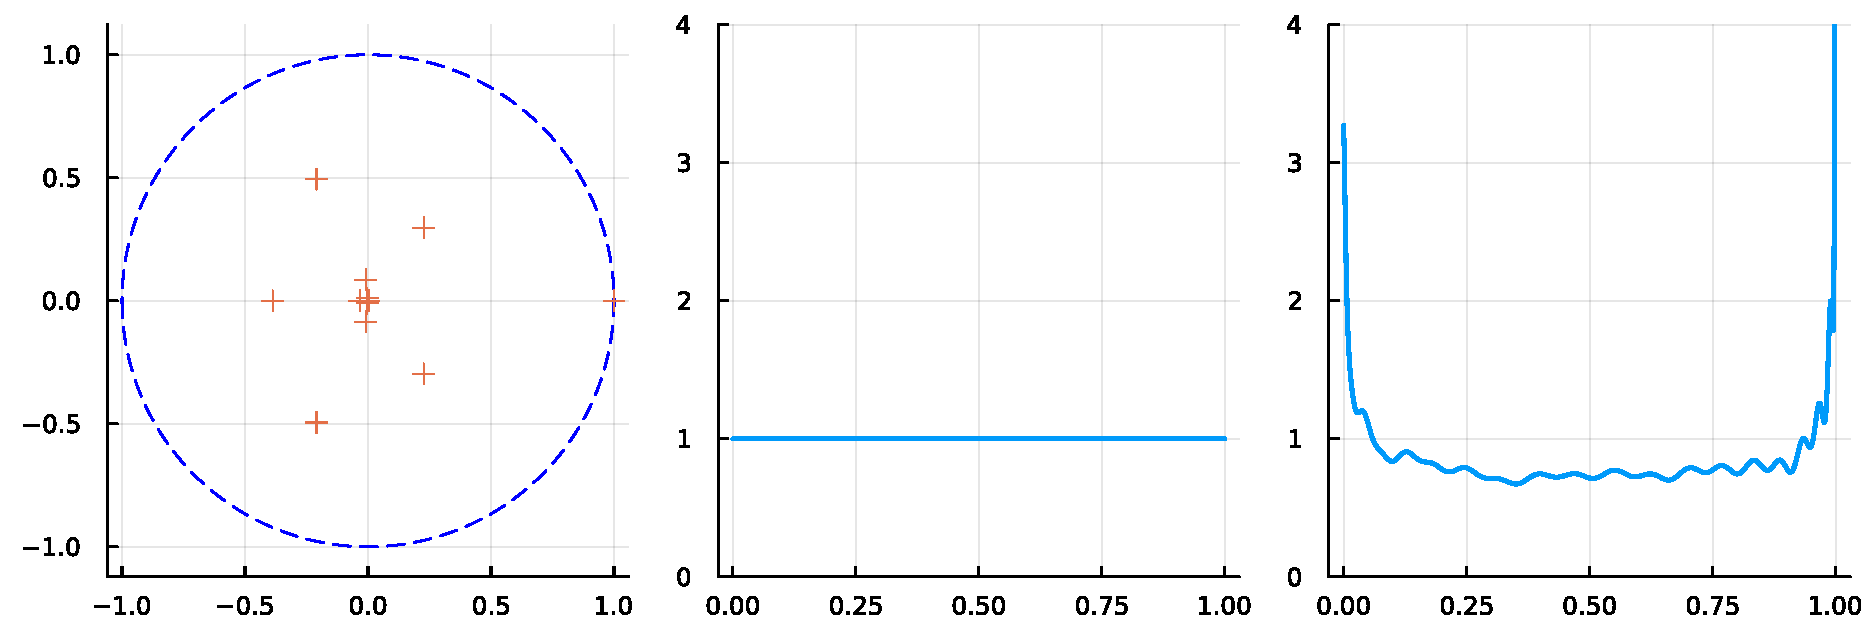
\includegraphics[width=\textwidth]{edmd.pdf}
    \caption{
        Algorithm \ref{alg:edmd} applied to the quadratic map (c.f. figure 
        \ref{fig:perron_asymptotic}) performed with $M = 100$ Gauß-Legendre quadrature 
        nodes and weights, and $N = 40$ Legendre polynomials transplanted to the interval 
        $[0, 1]$. Left: spectrum of $K$. Middle: (normalized) eigenfunction of $K$ for 
        the eigenvalue $\lambda = 1$. Right: (normalized) eigenfunction of $L$ for the 
        eigenvalue $\lambda = 1$. Compare with figure \ref{fig:quadratic_eigs}. 
    }\label{fig:edmd}
\end{figure}

% -------------------------------------------------------------------------------------- %

\subsubsection{EDMD for the Perron-Frobenius Operator}

From equation \ref{eq:functional_K}, and noting the form of $\bbA$, 
\begin{equation}
    \left\langle \psi_i, \scrL \psi_j \right\rangle 
    = \left\langle \scrK \psi_i, \psi_j \right\rangle 
    = \overline{ \left\langle \psi_j, \scrK \psi_i \right\rangle } 
    = \overline{\bbA_{j i}}
\end{equation}
yields an equivalent Galerkin method for $\scrL$:
\begin{equation}
    L = (\Psi^* \Psi)^{-1} \Psi^* (\scrL \Psi) = \bbG^{-1} \bbA^* 
\end{equation}
or the finite analogue:
\begin{equation}
    L = G^{-1} A^* . 
\end{equation}

\subsection{Residual EDMD (ResDMD)}

% -------------------------------------------------------------------------------------- %

\subsubsection{Validation of Koopman Eigenpairs}\label{sec:validation}

The formulation \ref{eq:PKP} shows that $K$ (when viewed as a operator on $\scrX$) 
converges weakly to $\scrK$. However, from example \ref{ex:spec_unstable} we know that 
the spectrum is already unstable for operators which are close in the \emph{strong} 
operator topology, let alone in the \emph{weak} topology. It is therefore entirely 
unclear \emph{a priori} that the eigenvalues and eigenvectors of $K$ actually represent 
eigenvalues and eigenfunctions of $\scrK$. 

In the Perron-Frobenius operator community, a common solution to the mentioned issue is 
\emph{stochastic blurring}. Instead of considering a deterministic dynamical system 
generated by $S$, one consider a stochastic system: $x \in \Omega$ is 
assigned a \emph{distribution} of possible image points instead of being assigned to 
the point $S(x)$. The resulting Markov process has an associated (stochastic) 
Perron-Frobenius operator which (under some conditions on the type of stochastic 
blurring) is Hilbert-Schmidt on $L^2 (\Omega)$. This way, the finite sections converge 
strongly to the (stochastic) Perron-Frobenius and (since it is Hilbert-Schmidt) so do 
the eigenvalues \cite{attr}. 

We take a different approach using the theory of pseudospectra. We wish to know which of 
our eigenvalues are \emph{spurious}, that is, caused by the reduction to a finite section, 
and which eigenvalues are accurate. To determine this, we consider equation 
\ref{eq:pseudospectrum}: if a sequence $(\lambda_N, c_N)_N$ of (normalized) eigenpairs for 
$K = K(\left\{ \psi_j \right\}_{j=1}^N)$ converges to a true $\lambda \in \sigma (\scrK)$ 
then we must have 
\begin{equation}
    \label{eq:true_residual}
    \lim_{N \to \infty} \left\| (\scrK - \lambda_N I) \Psi c_N \right\|_{\scrX}^2 = 0
\end{equation}
(where $\Psi = \Psi_N$ is as in \ref{eq:Psi}) or 
\begin{equation}
    \lim_{N \to \infty} \left\| (\scrL - \bar{\lambda}_N I) \Psi c_N \right\|_{\scrX}^2 = 0 . 
\end{equation}
Conversely, if neither of these tend to $0$ as $N$ grows, then we can rule out 
$\lambda_N$ as a candidate eigenvalue. 

From section \ref{sec:functional_minimization} we know that the Galerkin equation 
\ref{eq:edmd} is a quadrature approximation of equation \ref{eq:edmd_functional}. 
Similarly, the \emph{regression error}
\begin{equation}
    \label{eq:res}
    \res (\lambda, c; M, N)^2 \defeq \left\| \sqrt{W} (\YY - \lambda \YX) c \right\|_2^2
\end{equation}
is precisely a quadrature approximation of equation \ref{eq:true_residual}. 

\begin{theorem}
    \label{thm:res_M_limit}
    Let $\lambda$ and $g = \Psi c$ be a candidate eigenpair for $\scrK$. Then 
    \begin{equation}
        \lim_{M \to \infty} \res (\lambda, c; M, N)^2
        = \left\| (\scrK - \lambda I) g \right\|_{\scrX}^2
    \end{equation}
\end{theorem}

\begin{proof}
    Denote $J = \YY^* W \YY$ and observe that
    \begin{equation}
        \label{eq:J}
        \lim_{M \to \infty} J_{i j} = 
        \left\langle \scrK \psi_i, \scrK \psi_j \right\rangle \eqdef \bbJ_{i j} . 
    \end{equation}
    Consider the action of $\Psi$ on standard unit vectors:
    \begin{equation}
        \left\langle \Psi e_i, \Psi e_j \right\rangle 
        = \left\langle \psi_i, \psi_j \right\rangle 
        = \bbG_{i j} 
        = e_i^* \bbG e_j . 
    \end{equation}
    Analogously $e_i^* \bbA e_j = \left\langle \psi_i, \scrK \psi_j \right\rangle$, 
    $e_i^* \bbJ e_j = \left\langle \scrK \psi_i, \scrK \psi_j \right\rangle$. 
    Sesquilinearity of $\left\langle \cdot, \cdot \right\rangle$ yields 
    \begin{equation}
        \left\langle g, g \right\rangle = c^* \bbG c, \quad 
        \left\langle g, \scrK g \right\rangle = c^* \bbA c, \quad 
        \left\langle \scrK g, \scrK g \right\rangle = c^* \bbJ c . 
    \end{equation}
    The proof is now simply a calculation. Indeed,
    \begin{equation}
        \label{eq:reg_error}
        \begin{split}
            &\left\| \sqrt{W} ( \YY - \lambda \YX ) c \right\|_2^2 \\[1ex]
            &= \left(\, ( \YY - \lambda \YX ) c \,\right)^* \,W\, \left(\, ( \YY - \lambda \YX ) c \,\right) \\[1ex]
            &= c^* \left(\, 
                \YY^* W \YY - \bar{\lambda} \YX^* W \YY - \lambda \YY^* W \YX + | \lambda |^2 \YX^* W \YX \,\right) c \\[1ex]
            &= c^* J c \,-\, \bar{\lambda}\, c^* A c \,-\, \lambda\, c^* A^* c \,+\, | \lambda |^2\, c^* G c . 
        \end{split}
    \end{equation}
    Taking the infinite-data limit,
    \begin{equation}
        \label{eq:residual}
        \begin{split}
            \lim_{M \to \infty} & \left\| \sqrt{W} ( \YY - \lambda \YX ) c \right\|_2^2 \\[1ex]
            &= c^* \bbJ c \,-\, \bar{\lambda} \,c^* \bbA c \,-\, \lambda\, c^* \bbA^* c \,+\, | \lambda |^2\, c^* \bbG c \\[1.2ex]
            &= \left\langle \scrK g, \scrK g \right\rangle
            - \bar{\lambda} \left\langle g, \scrK g \right\rangle
            - \lambda \left\langle \scrK g, g \right\rangle
            + | \lambda |^2 \left\langle g, g \right\rangle \\[1.2ex]
            &= \left\langle \left( \scrK - \lambda I \right) g, 
            \left( \scrK - \lambda I \right) g \right\rangle \\[1.2ex]
            &= \left\| \left( \scrK - \lambda I \right) g \right\|_{\scrX}^2 . 
        \end{split}
    \end{equation}
\end{proof}

From the proof we also directly see the following corollaries. 

\begin{definition}
    Let $M : \scrX \supset D(M) \to \scrY$ be a closed linear operator and 
    $V \subset \scrX$. We say that $V$ forms a \emph{core} of $M$ if the closure\footnote{
        A linear operator $N : D(N) \to \scrY$ which is \emph{not} closed might only be so 
        because the domain $D(N)$ might not be "large enough". If there exists an extension 
        (i.e. $\bar{N} : D(\bar{N}) \to \scrY$, $D(N) \subset D(\bar{N})$, 
        $\left. \bar{N} \right|_{D(N)} = N$) which is closed, then $N$ is \emph{closable} and 
        the smallest such $\bar{N}$ is called the \emph{closure} of $N$. 
    } 
    of $\left. M \right|_{V}$ if $M$. 
\end{definition}

\begin{corollary}
    Let $\lambda \in \bbC$, define
    \begin{equation}
        \res (\lambda; M, N)
        \defeq \min_{c^* G c = 1} \res (\lambda, c; M, N) . 
    \end{equation} 
    Then
    \begin{equation}
        \label{eq:resdmd_M_limit}
        \lim_{M \to \infty} \res (\lambda; M, N)
        = \min_{\substack{g \in \spn \left\{ \psi_1, \ldots, \psi_N \right\} \\ \| g \| = 1}}
            \left\| ( \scrK - \lambda I ) g \right\|_\scrX . 
    \end{equation}
\end{corollary}

In particular this corollary implies that if we calculate some candidate eigenpairs, 
compute $\res$ for each one, and throw out eigenpairs which do not satisfy 
a threshhold $\res (\lambda, c) < \epsilon$, then the remaining candidate 
eignpairs really are close to eigenpairs of $\scrK$. This process is summarized in 
algorithm \ref{alg:edmd_verified_residual}. 

\begin{corollary}
    Let $\Lambda (\epsilon; M, N)$ denote the set of eigenvalues returned by algorithm 
    \ref{alg:edmd_verified_residual}. Then 
    \begin{equation}
        \limsup_{M \to \infty} \max_{\lambda \in \Lambda (\epsilon; M, N)}
        \left\| (\scrK - \lambda I)^{-1} \right\|^{-1} \leq \epsilon . 
    \end{equation}
\end{corollary}

Finally, theorem \ref{thm:res_M_limit} also provides a method to compute the 
$\epsilon$-approximate point pseudospectrum of $\scrK$, summarized in 
algorithm \ref{alg:resdmd}. 

\begin{corollary}
    \label{cor:K_ap_epsilon}
    Assume $\spn \left\{ \psi_j \right\}_{j=1}^\infty$ forms a core of $\scrK$. 
    Then
    \begin{equation}
        \lim_{N \to \infty} \lim_{M \to \infty} \res (\lambda; M, N) 
        = \sigma_{\inf} (\scrK - \lambda I) . 
    \end{equation}
    Moreover the outer limit $N \to \infty$ is monotonically decreasing so that 
    \begin{equation}
        \sigma_{ap, \epsilon} (\scrK) = 
        \bigcap_{N > 0} \left\{ \lambda \in \bbC \mid 
        \lim_{M \to \infty} \res (\lambda; M, N) < \epsilon \right\} . 
    \end{equation}
\end{corollary}

\begin{proof}
    From \ref{eq:resdmd_M_limit} it is clear that 
    $\lim_{M \to \infty} \res_{N,M} (\lambda) \geq \sigma_{\inf} (\scrK - \lambda I)$
    and that $\res_{N,M}$ is decreasing with $N$. Let $\delta > 0$ be arbitrary and 
    $g \in \scrX$ be such that $\|g\|=1$ and 
    $\left\| (\scrK - \lambda I) g \right\| < \sigma_{\inf} (\scrK - \lambda I) + \delta$. 
    Since $\spn \left\{ \psi_j \right\}_{j=1}^\infty$ forms a core of $\scrK$, 
    we can find an $N$ and $\widehat{g} \in \spn \left\{ \psi_j \right\}_{j=1}^N$ 
    such that $\| g - \widehat{g} \| < \delta$ and 
    $\left\| (\scrK - \lambda I) \widehat{g} \right\| < 
    \left\| (\scrK - \lambda I) g \right\| + \delta$. This implies 
    $\| \widehat{g} \| > 1- \delta$ and $\left\| (\scrK - \lambda I) \widehat{g} \right\| < 
    (\sigma_{\inf} (\scrK - \lambda I) + 2\epsilon) / (1 - \epsilon)$. Since this holds 
    for all $\epsilon > 0$, the claim is proven. In fact, the convergence is uniform on 
    compact sets. 
\end{proof}

The computation of $\res (\lambda)$ reduces to a generalized eigenvalue problem. Let 
\begin{equation}
    U \,( = U(\lambda) )\, = J - \bar{\lambda} A - \lambda A^* + | \lambda |^2 G . 
\end{equation}
Then computing $\res (\lambda)^2$ is equivalent to solving the minimization problem 
\begin{equation}
    \label{eq:res_min}
    \min_{c \in \bbC^N} c^* U c \quad \text{ such that } \quad c^* G c = 1 .  
\end{equation}
Let $\xi$ be a Lagrange multiplier, that is, a necessary condition for a solution of 
\ref{eq:res_min} is 
\begin{equation}
    \label{eq:generalized_eig}
    U c - \xi G c = 0 
\end{equation}
since $U$ and $G$ are (conjugate) symmetric. Inserting such a $c$ into the objective yields 
\begin{equation}
    c^* U c = c^* \xi G c = \xi
\end{equation}
since $c^* G c = 1$. Hence \ref{eq:res_min} is solved by computing the smallest 
generalized eigenvalue solution of \ref{eq:generalized_eig} (symmetry of $U$ and $G$ 
guarantees that all such eigenvalues are real). 

\begin{algorithm}
    \caption{Verification of candidate eigenpairs for $\scrK$}
    \label{alg:edmd_verified_residual}
    \begin{algorithmic}[1]
        \Require Dictionary $\left\{ \psi_j \right\}_{j=1}^N$, 
            data points and weights $\left\{ (w_i, x_i) \right\}_{i=1}^M$, 
            tolerance $\epsilon$
        \State Perform algorithm \ref{alg:edmd} to obtain $G$, $A$, $K V = V \Lambda$
        \State Construct $J$ as in \ref{eq:J}
        \For{each candidate eigenpair $(\lambda, v)$}
            \State Compute $\res (\lambda, v)$ as in \ref{eq:res_min}
            \State Throw out $\lambda$ if $\res (\lambda, v) \geq \epsilon$
        \EndFor
        \State \Return Verified Koopman (approximate-point) eigenvalues 
        $\Lambda (\epsilon; M, N) = \left\{ (\lambda, v) \mid \res (\lambda, v) < \epsilon \right\}$
    \end{algorithmic}
\end{algorithm}

\begin{algorithm}
    \caption{Residual EDMD to Compute $\sigma_{ap, \epsilon} (\scrK)$}
    \label{alg:resdmd}
    \begin{algorithmic}[1]
        \Require Dictionary $\left\{ \psi_j \right\}_{j=1}^N$, 
            data points and weights $\left\{ (w_i, x_i) \right\}_{i=1}^M$, 
            grid $\left\{ z_\nu \right\}_{\nu=1}^T \subset \bbC$,
            tolerance $\epsilon$
        \State Perform algorithm \ref{alg:edmd} to obtain $G$, $A$, $K$
        \State Construct $J$ as in \ref{eq:J}
        \For{$z_\nu$}
            \State Compute $\res (z_\nu)$ as in \ref{eq:res_min}
        \EndFor
        \State \Return $\left\{ z_\nu \mid \res (z_\nu) < \epsilon \right\}$
            as an approximation for $\sigma_{ap, \epsilon} (\scrK)$
    \end{algorithmic}
\end{algorithm}

\begin{figure}
    \centering
    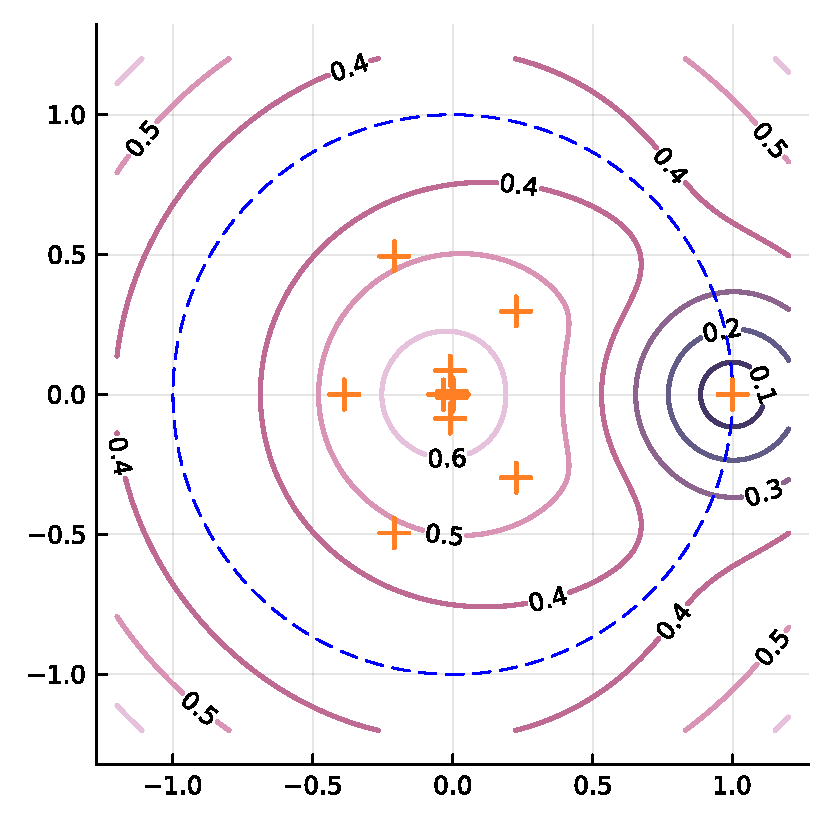
\includegraphics[width=0.5\textwidth]{resdmd.pdf}
    \caption{
        Algorithm \ref{alg:resdmd} applied to the quadratic map (c.f. figure 
        \ref{fig:perron_asymptotic}) performed with the same parameters as 
        figure \ref{fig:edmd}. Contours of $\lambda \mapsto \res (\lambda)$ are shown with 
        the spectrum of $K$. The quadratic map is ergodic \cite{logisitc_ergodic} 
        which is verified by the residuals. The eigenvalues of $K$ other than $1$ 
        are spurious. 
    }\label{fig:resdmd}
\end{figure}

% -------------------------------------------------------------------------------------- %

\subsubsection{A Naive Attempt at Duality}

From this point onward, we shall always assume (without loss of generality) that $\YX$ has 
full rank, that is, rank $N$ when $N \leq M$ or rank $M$ when $M \leq N$. 

Algorithm \ref{alg:resdmd} provides a way to compute the approximate-point pseudospectrum 
of the Koopman operator. In order to resolve the full pseudospectrum, one needs to compute 
$\sigma_{\inf} (\scrK - \lambda I)$ \emph{and} $\sigma_{\inf} (\scrL - \bar{\lambda} I)$ 
for $\lambda$'s of interest. One could hope to perform the calculations in \ref{eq:residual} 
backwards using $\scrL$ instead of $\scrK$, but quickly notices that the inner product 
$\left\langle \scrL g, \scrL g \right\rangle$ or $g = \Psi c$ is not computable using just 
the information at hand. 

We instead try to follow the calculations forward. Starting with $L = G^{-1} A^*$ 
and $g = \Psi c$ we see that the analogous regression error for a candidate eigenpair can 
be written as 
\begin{equation}
    \left\| \left( A^* - \lambda G \right) c \right\|_{\bbC^N}^2 
    = \left\| \left( \YY^* W - \lambda \YX^* W \right) \YX c \right\|_{\bbC^N}^2 . 
\end{equation}
Notice that $\YX^* W$ is precisely a quadrature appoximation of $\Psi^*$ from equation 
\ref{eq:Psi_star}. $\YX^* W$ takes an interpolation vector $f \in \bbC^M$ and 
approximates the inner product with an interpolant function. Analogously we can deduce that 
$\YY^* W$ is a quadrature approximation of $(\scrK \Psi)^*$. 

Assuming that $\left\{ \psi_j \right\}_{j=1}^N$ is an orthonormal family, taking the 
infinite data limit yields
\begin{equation}
    \label{eq:bad_L_pseudospectrum}
    \begin{split}
        \lim_{M \to \infty} &
        \left\| \left( \YY^* W - \lambda \YX^* W \right) \YX c \right\|_{\bbC^N}^2 \\
        &= \left\| \left( (\scrK \Psi)^* - \lambda \Psi^* \right) g \right\|_{\bbC^N}^2 \\
        &= \left\| \begin{pmatrix}
            \left\langle\, (\scrK - \lambda I) \psi_1, g \,\right\rangle \\
            \vdots \\
            \left\langle\, (\scrK - \lambda I) \psi_N, g \,\right\rangle 
        \end{pmatrix} \right\|_{\bbC^N}^2 \\
        &= \sum_{j=1}^{N} \left| \left\langle\, (\scrK - \lambda I) \psi_j, g \,\right\rangle \right|^2 \\
        &= \sum_{j=1}^{N} \left| \left\langle\, \psi_j, (\scrL - \bar{\lambda} I) g \,\right\rangle \right|^2 \\
        &= \left\| (\Pi \scrL \Pi - \bar{\lambda} I) g \right\|_{\scrX}^2
    \end{split}
\end{equation}
where $\Pi$ is the orthogonal projector onto $\spn \left\{ \psi_j \right\}_{j=1}^N$. By 
the Galerkin property we know that $L$ encodes precisely the action of $\Pi \scrL \Pi$. Hence, 
\begin{equation}
    \label{eq:PLP}
    \left\| (\Pi \scrL \Pi - \bar{\lambda} I) g \right\|_{\scrX}^2
    = \left\| (L - \bar{\lambda} I) c \right\|_{\bbC^N}^2 
\end{equation}
and so the least-squares Ansatz computes the pseudospectrum of $L$ which by theorem 
\ref{thm:projection_pseudospectrum} 
cannot be used analogously to algorithm \ref{alg:resdmd} to compute 
$\sigma_{ap,\epsilon} (\scrL)$. We would need to send $N \to \infty$ before $N \to \infty$, 
which would cause the equation $L = G^{-1} A^*$ to break. 

While we will not use this immediately, we still expand the first line of 
\ref{eq:bad_L_pseudospectrum} since we will see it again later. 
\begin{equation}
    \label{eq:L_res_expanded}
    \begin{split}
        &\left\| \left( \YY^* W - \lambda \YX^* W \right) \YX c \right\|_{\bbC^N}^2 \\
        &= \left\| \left( \YY^* \sqrt{W} - \lambda \YX^* \sqrt{W} \right) \sqrt{W} \YX c \right\|_{\bbC^N}^2 \\
        &= \left( \sqrt{W} \YX c \right)^*
        \sqrt{W} \left( 
            \YY \YY^* - \bar{\lambda} \YX \YY^* - \lambda \YY \YX^* \right. \\
            & \quad\quad\quad\quad\quad\quad\quad\quad\quad\quad\quad\quad
            \left. + | \lambda |^2 \YX \YX^*
        \right) \sqrt{W}
        \left( \sqrt{W} \YX c \right)
    \end{split}
\end{equation}


\subsection{kernel EDMD (kEDMD)}

% -------------------------------------------------------------------------------------- %

\subsubsection{The Kernel Trick and Reproducing Kernel Hilbert Spaces}

The choice of dictionary $\left\{ \psi_j \right\}_{j=1}^N$ naturally has massive impacts 
on the accuracy of the above methods. We will see later in section \ref{sec:benchmark} 
that a poorly chosen dictionary can cause catastrophic results. This is because even 
though there may be many ways to (in the limit $N \to \infty$) form a basis of $\scrX$, 
any practical calculation will necessarily have a finite cut-off. So the challenge 
becomes finding efficient ways to increase $N$ without needing to perform $O(N^2)$ 
quadrature problems. 

One method which is enormously popular in machine learning 
\cite{kernel_OG,campbell2001,hofmann2008,muller2018}
is the so-called \emph{kernel trick}. Consider the function 
$k : \bbC^2 \times \bbC^2 \to \bbC,\ (w,z) \mapsto (1 + w^* z)^2$. We can write this as 
\begin{equation}
    \begin{split}
        k(w, z) &= (1 + \bar{w_1} z_1 + \bar{w_2} z_2)^2 \\
        &= (1 + 2 \bar{w_1} z_1 + 2 \bar{w_2} z_2 + 2 \bar{w_1} \bar{w_2} z_1 z_2 + \bar{w_1}^2 z_1^2 + \bar{w_2}^2 z_2^2) \\
        &= \left\langle \Psi (z), \Psi (w) \right\rangle_{\bbC^{1 \times 6}}\ (= \Psi (z) \Psi (w)^*)
    \end{split}
\end{equation}
for the basis 
\begin{equation}
    \Psi (x) = \left[ 
        1 \ \big|\ 
        \sqrt{2} x_1 \ \big|\ 
        \sqrt{2} x_2 \ \big|\ 
        \sqrt{2} x_1 x_2 \ \big|\ 
        x_1^2 \ \big|\ x_2^2 
    \right] \in \bbC^{1 \times 6} . 
\end{equation}
While the result is the same, computation of $(1 + w^* z)^2$ requires only $5$ 
floating-point operations, whereas $\Psi (z) \Psi (w)^*$ requires $23$. More generally, 
any such relation $k(w, z) = \Psi (z) \Psi (w)^*$ is called a kernel trick. 

\begin{definition}
    Let $k : \Omega \times \Omega \to \bbC$ be 
    \begin{enumerate}
        \item continuous,
        \item \emph{conjugate-symmetric}, i.e. $k(w, z) = \overline{k(z, w)}$,
        \item \emph{finitely positive semidefinite}, i.e. for all 
            $x_1, \ldots, x_M \in \Omega$ 
            the matrix $\bbG = (\, k(x_j, x_k) \,)_{j,k=1}^M \in \bbC^{M \times M}$ 
            is positive semidefinite\footnote{
                For any $v \in \bbC^M$, $v^* \bbG v \geq 0$. 
            }. 
    \end{enumerate}
    Then $k$ is called \emph{valid} or \emph{Mercer} kernel. 
    A function $\Psi : \Omega \to \scrY$ into some Hilbert space $\scrY$ with 
    $k(w, z) = \left\langle \Psi (z), \Psi (w) \right\rangle_\scrY$ is known as a 
    \emph{feature map}. 
\end{definition}

One obvious kernel is given by a dictionary: letting 
$\Psi (x) = \left[ \psi_1 (x) \mid \ldots \mid \psi_N (x) \right]$ as before, 
$k(w, z) = \Psi (z) \Psi (w)^*$ is also a kernel. Moreover, one sees that when 
$k(z, \cdot)$ is an element of some Hilbert space $\scrY$, then another 
obvious feature map is given by $\Psi (z) = k(z, \cdot)$. This feature map (called 
\emph{canonical} feature map) is of much importance. This is because the functions 
which can be represented by the features are precisely of this form. 

\begin{definition}
    A Hilbert space $\scrY$ which enjoys the \emph{reproducing property}: 
    \begin{enumerate}
        \item $k (w, \cdot) \in \scrY$ for all $w \in \Omega$,
        \item $\left\langle k(w, \cdot), f \right\rangle = f (w)$ for all 
            $f \in \scrY$
    \end{enumerate}
    is called \emph{reproducing kernel Hilbert space (RKHS)} generated by $k$. 
\end{definition}

The following are immediate from the definition:

\begin{lemma}
    Let $k$ generate a RKHS $\scrY$. Then
    \begin{enumerate}
        \item $\left\langle k(w, \cdot), k(\cdot, z) \right\rangle_\scrY = k(w, z)$ 
            for all $w, z \in \Omega$,
        \item The set $\left\{ k(w, \cdot) \mid w \in \Omega \right\}$ is 
            dense in $\scrY$ (w.r.t. the $\scrY$-norm). 
    \end{enumerate}
\end{lemma}

We conclude the list of basic facts about RKHS with a characterization of 
when a kernel generates an RKHS. The following is a special case of theorem 
$4$ from \cite{RKHS_probability}. 

\begin{theorem}
    \label{thm:RKHS}
    Let $\Omega$ be compact, $k : \Omega \times \Omega \to \bbC$ continuous on the 
    finite measure space $(\Omega, dx)$. Then the following are equivalent: 
    \begin{enumerate}
        \item $k$ is finintely positive semidefinite. 
        \item $k$ is the kernel of some unique RKHS $\scrH \subset \scrC^0$, where $\scrC^0$ 
            denotes the set of continuous functions on $\Omega$. 
        \item $k$ is of the form 
            \begin{equation}
                k(w, z) 
                = \sum_{j=1}^{\infty} \mu_j^2\, \phi_j (z) \overline{\phi_j (w)}
                = \Psi (z) \Psi (w)^*
            \end{equation}
            for $\Psi (z) = \left[ \mu_1 \phi_1 \mid \mu_2 \phi_2 \mid \ldots \right]$. 
            The set $\left\{ \phi_j \right\}_{j=1}^\infty$ forms an orthonormal 
            basis of $L^2 (\Omega)$. 
            The $\mu_j \geq 0$ can be ordered by decreasing magnitude and 
            converge to $0$ as $j \to \infty$. 
    \end{enumerate}
    Moreover, the set $\left\{ \psi_j \defeq \mu_j \phi_j \right\}_{j=1}^\infty$
    forms an orthonormal basis of $\scrH$. 
\end{theorem}

Entire books are written on such kernels \cite{RKHS} and their properties. Common 
kernels include:

\begin{example}
    The \emph{polynomial kernel} 
    $k : \bbC^d \times \bbC^d \to \bbC,\ (w, z) \mapsto (1 + w^* z / c^2)^\alpha$ 
    feature map is given by all (multivariate) polynomials up to degree $\alpha$. Note 
    that computing $k(w, z)$ requires only $O(d)$ operations, but computing 
    $\Psi (z) \Psi (w)^*$ requires superexponentially (in $\alpha$) many combinations. 
\end{example}

\begin{example}
    The \emph{Gaußian kernel} 
    $k(w, z) = \exp \left( -\frac{\left\| w - z \right\|^2}{c^2} \right)$, $c \neq 0$, has a feature 
    map which is infinite-dimensional. Indeed, consider (for notational simplicity) 
    $w, z \in \bbR$: 
    \begin{equation}
        \label{eq:gauss_kernel_calc}
        \begin{split}
            k(w, z) &= 
            \exp \left( -\frac{| w |^2}{c^2} \right) \cdot
            \exp \left( \frac{2\, w \cdot z}{c^2} \right) \cdot
            \exp \left( -\frac{| z |^2}{c^2} \right) \\
            &= \exp \left( -\frac{| w |^2}{c^2} \right) \cdot
            \left( \sum_{k=0}^{\infty} \frac{1}{k!} \left( \frac{2}{c^2} \right)^k (w \cdot z)^k \right)
            \cdot \exp \left( -\frac{| z |^2}{c^2} \right)
        \end{split}
    \end{equation}
    so that 
    \begin{equation}
        \Psi (x) = 
        \exp \left( -\frac{| x |^2}{c^2} \right)
        \left[ 
            1 \ \ \Bigg|\ \ 
            \frac{\sqrt{2}}{c} x \ \ \Bigg|\ \ 
            \frac{1}{\sqrt{2 !}} \left( \frac{\sqrt{2}}{c} x \right)^2 \ \ \Bigg|\ \ 
            \ldots 
        \right] . 
    \end{equation}
    When $w, z \in \bbC$ then the middle term in \ref{eq:gauss_kernel_calc} changes from 
    $w \cdot z$ to $\bar{w} \cdot z + \bar{z} \cdot w$, and in higher dimensions this 
    extends to all pairwise combinations of the components of $w$ and $z$. We note 
    (and will use later) that the Gaußian kernel is \emph{universal}, meaning the RKHS 
    $\scrH$ generated by $k$ is dense in $\scrC^0$. 
\end{example}

\begin{example}
    The Sobolev space $H^s$ contains all functions which are square integrable and whose 
    (weak) derivatives up to oder $s$ are also square integrable. That is, $H^s$ is the 
    closure of the smooth functions with compact support $\scrC^\infty_c$ with respect 
    to the norm 
    \begin{equation}
        \left\| f \right\|_{H^s}^2 = 
        \sum_{| \alpha | \leq s} \left\| D^\alpha f \right\|_{L^2}^2
    \end{equation}
    where $\alpha \in \bbN_0^d$ are multiindices. 
    Using the Fourier transform $\scrF$ this can readily be rewritten as 
    $\left\| f \right\|_{H^s}^2 = \left\langle f, f \right\rangle_{H^s}$ for
    \begin{equation}
        \left\langle f, g \right\rangle_{H^s} = 
        \int \left( 1 + \left| \xi \right|^2 \right)^s 
        \,\overline{ \scrF f (\xi) }\, \scrF g (\xi) \ dx . 
    \end{equation}
    It can be shown \cite{RKHS} that the kernel 
    \begin{equation}
        k : \bbC^d \times \bbC^d \to \bbC, \quad (w, z) \mapsto 
        (2 \pi)^{-d} \int \left( 1 + \left| \xi \right|^2 \right)^{-s} 
        \exp \left( i (w - z) \cdot \xi \right) \,d\xi 
    \end{equation}
    generates $H^s$. Moreover, when $d=1$ and $\Omega = [a, b]$ is an interval, the 
    \emph{Laplace kernel} 
    \begin{equation}
        k : [a,b] \times [a,b] \to \bbR, \quad (w, z) \mapsto 
        \frac{1}{2} \exp ( - \left| w - z \right| )
    \end{equation}
    generates the slightly altered Sobolev norm
    \begin{equation}
        \left\| f \right\|_{\tilde{H}^2}^2 = \left\| f \right\|_{H^2}^2 
        + \left| f(a) \right|^2 
        + \left| f(b) \right|^2 . 
    \end{equation}
    Note that \emph{as sets}, $\tilde{H}^2 = H^2$. 
\end{example}

% -------------------------------------------------------------------------------------- %

\subsubsection{Application to EDMD}

%Let $k$ be a kernel with associated feature map $\Psi$ that is rescaled such that 
%\begin{equation}
%    \Psi (x_j) \Psi (x_i)^* = \frac{k(x_i, x_j)}{\sqrt{w_i w_j}} \quad 
%    \text{for all } 1 \leq i, j \leq M . 
%\end{equation} 
%In most cases $w_i = 1/M$ for all $i$ so that the kernel is just scaled by a constant 
%factor $1/M$. 

Notice that 
\begin{equation}
    G = \YX^* W \YX = \sum_{i=1}^{M} w_i\, \Psi (x_i)^* \Psi (x_i), \quad
    A = \YX^* W \YY = \sum_{i=1}^{M} w_i\, \Psi (x_i)^* \Psi (S(x_i)) . 
\end{equation}
Each summand is a rank one matrix in $\bbC^{N \times N}$. $N$ might be infinite, in which 
case we interpret this statement as being about "infinite matrix" type operators in $\ell^2$. 

This is not in a form where one could use the kernel trick, since we have summands of the 
form $\Psi (x_i)^* \Psi (x_i)$ instead of $\Psi (x_i) \Psi (x_i)^*$. However, if we 
reverse the order of multiplication in $\YX^* W \YX = (\sqrt{W} \YX)^* (\sqrt{W} \YX)$ 
then 
\begin{equation}
    \label{eq:G_hat}
    \begin{split}
        \widehat{G} &= \sqrt{W} \Psi_X \Psi_X^* \sqrt{W} \\
        &= \left(\; \sqrt{w_j w_i} \cdot \Psi (x_j) \Psi (x_i)^* \;\right)_{i, j=1}^M \\
        &= \left(\; \sqrt{w_i w_j} \cdot k(x_i, x_j) \;\right)_{i, j=1}^M . 
    \end{split}
\end{equation}
Analogously 
\begin{equation}
    \label{eq:A_hat}
    \widehat{A} = \sqrt{W} \Psi_Y \Psi_X^* \sqrt{W}
    = \left(\; \sqrt{w_i w_j} \cdot k(S(x_i), x_j) \;\right)_{i, j=1}^M . 
\end{equation}
We would now like to exploit the form of $K = \YX^\dagger \YY$ 
to use these "flipped" matrices. The key to do so will be a (compact) singular value 
decomposition
\begin{equation}
    \label{eq:psi_x_svd}
    \sqrt{W} \YX = Q \Sigma Z^*
\end{equation}
where $r = \min\{M, N\}$, $\Sigma \in \bbR_{\geq 0}^{r \times r}$ is a nonnegative diagonal 
matrix, and $Q \in \bbC^{M \times r}$ and $Z \in \bbC^{N \times r}$ are semi-unitary\footnote{
    A tall martrix $M \in \bbC^{q \times r}$, $q \geq r$, is semi-unitary if the columns 
    form an orthonormal family. 
}. 

\begin{theorem}
    \label{thm:K_hat}
    Let 
    \begin{equation}
        \label{eq:K_hat}
        \widehat{K} \defeq 
        \left( \Sigma^\dagger Q^* \right) \widehat{A} \left( Q \Sigma^\dagger \right) . 
    \end{equation}
    Then 
    \begin{equation}
        \label{eq:K_hat_K}
        \widehat{ K } = Z^* K Z
    \end{equation}
    and when $N \leq M$, 
    \begin{equation}
        \widehat{ K }^* = \left( \Sigma^2 Z^* \right) L \left( Z \Sigma^{-2} \right) . 
    \end{equation}
    In particular, equation \ref{eq:K_hat_K} shows that
    a pair $(\lambda, v) \in \bbC \times \bbC^r$ (for $\lambda \neq 0$) 
    is an eigenpair of $\widehat{K}$ iff $(\lambda, Z v) \in \bbC \times \bbC^N$ is an 
    eigenpair of $K$. Moreover, the eigenmodes $g = \Psi \cdot (Z v)$ can be evaluated 
    at the data points $x_i$, $i = 1, \ldots M$. 
\end{theorem}

One should take a moment to consider that the last statement made in the theorem
seems highly nontrivial at first. Often, the feature map is only given implicitly - one knows 
there exists such a $\Psi$, but does not have an explicit form. Even worse, the matrix 
$Z$ is completely unatainable from just $\widehat{G}$ and $\widehat{A}$. 

The benefit of using $\widehat{K}$ is that it can be computed in $O(M^2)$ time, 
\emph{independent of $N$}. All that is required is an eigendecomposition for $\widehat{G}$ 
since by definition 
\begin{equation}
    \widehat{G} = Q \Sigma^2 Q^* . 
\end{equation} 

\begin{proof}
    Notice
    \begin{equation}
        Z \widehat{ K } Z^* 
        = \YX^\dagger \sqrt{W}^{-1} \sqrt{W} \YY \YX^* \sqrt{W} \sqrt{W}^{-1} {\YX^*}^\dagger%\left( \left( \sqrt{W} \YX \right)^* \right)^\dagger 
        = K \Pi_{\ran\, \YX^* \sqrt{W}}
    \end{equation}
    where $\Pi_{\ran \YX^* \sqrt{W}}$ is the orthogonal projection onto the range of $\YX^* \sqrt{W}$. 
    But since $\YX^* \sqrt{W} = Z \Sigma Q^*$, this is equivalent to 
    \begin{equation}
        \label{eq:Z*_K_Z}
        \widehat{ K } = Z^* K Z . 
    \end{equation}
    Now 
    \begin{equation}
        \begin{split}
            \widehat{ K }^* &= Z^* K^* Z \\
            &= Z^* A^* G^{-1} Z \\
            &= Z^* G G^{-1} A^* G^{-1} Z \\
            &= \left( Z^* G \right) L \left( G^{-1} Z \right) \\
            &= \left( \Sigma^2 Z^* \right) L \left( Z \Sigma^{-2} \right)
        \end{split}
    \end{equation}
    where we used that $G$ is symmetric and (when $N \leq M$) invertible.  

    Finally, to evaluate $g = \Psi \cdot (Z v)$ at each $x_i$, $i = 1, \ldots, M$, 
    observe that $\YX \cdot (Z v) = Q \Sigma v$. 
\end{proof}

\begin{algorithm}
    \caption{Kernel EDMD}
    \label{alg:kedmd}
    \begin{algorithmic}[1]
        \Require kernel $k : \Omega \times \Omega \to \bbC$, data points and weights 
            $\left\{ (w_i, x_i) \right\}_{i=1}^M$, compression factor $r \leq M$
        \State Construct $\widehat{G}$, $\widehat{A}$ as in \ref{eq:G_hat}, \ref{eq:A_hat}
        \State Compute an eigendecomposition $\widehat{G} = Q \Sigma^2 Q^*$
        \State Let $\widetilde{\Sigma} = \Sigma [1:r, 1:r]$, $\widetilde{Q} = Q [:, 1:r]$ be the 
            $r$ largest eigenvalues and corresponding eigenvectors
        \State Construct 
        $\widehat{K} = 
        \left( \widetilde{\Sigma}^\dagger \widetilde{Q}^* \right)
        \widehat{A}
        \left( \widetilde{Q} \widetilde{\Sigma}^\dagger \right)$
        \State Compute an eigendecomposition $\widehat{K} V = V \Lambda$
        \State \Return Eigenvalues and eigenvectors $\Lambda$, $V$
    \end{algorithmic}
\end{algorithm}

\subsection{kernel ResDMD (kResDMD)}

% -------------------------------------------------------------------------------------- %

\subsubsection{Associating a Residual to $\widehat{K}$}

We set out again to deduce which candidate eigenvalues produced by algorithm 
\ref{alg:kedmd} are spurious, and which are accurate. Theorem \ref{thm:K_hat} suggests 
that we could potentially compute $\| (\scrK - \lambda I) g \|$ by using the altered 
features $g = \Psi \cdot (Z v)$ the same way as in theorem \ref{thm:res_M_limit}. However, 
this is not effective in the regime $M \leq N$ (remember that the benefit of kernel 
methods was the ability to cheaply crank $N$ up). 

\begin{proposition}[\cite{resdmd}]
    Suppose $M \leq N$ and $\sqrt{W} \YX \in \bbC^{M \times N}$ has full rank. Then 
    for any eigenpair $(\lambda, v)$ of $\widehat{K}$, the residual
    \begin{equation}
        \res (\lambda, Z v; M, N) = 0 . 
    \end{equation}
\end{proposition}

\begin{proof}
    Write
    \begin{equation}
        \sqrt{W} (\YY - \lambda \YX) (Z v) 
        = \sqrt{W} \YY Z c - \lambda Q \Sigma v
        = \sqrt{W} \YY \YX^* \sqrt{W} Q \Sigma^\dagger c - \lambda Q \Sigma v . 
    \end{equation}
    Since $\sqrt{W} \YX$ has full rank, the singular value matrix $\Sigma$ in 
    $\sqrt{W} \YX = Q \Sigma Z^*$ is invertible, and so 
    $\sqrt{W} \YY \YX^* \sqrt{W} Q \Sigma^\dagger = Q \Sigma \widehat{K}$. Inserting, we see 
    \begin{equation}
        \sqrt{W} (\YY - \lambda \YX) (Z v) = Q \Sigma (\widehat{K} - \lambda I) v = 0 .  
    \end{equation}
\end{proof}

The proposition suggests that we are suffering from \emph{overfitting} of the snapshot 
data. We therefore require a different way to associate a residual to the eigenpair. 

Recall from equation \ref{eq:res} that $\res$ has an alternative representation as 
a regression error. We could analogously ask if $\widehat{K}$ is the solution of a different 
regression problem. 

Let 
\begin{equation}
    \widehat{\YX} = \left( \sqrt{W} \YX \right)^* Q \Sigma^\dagger = Z, \quad 
    \widehat{\YY} = \left( \sqrt{W} \YY \right)^* Q \Sigma^\dagger . 
\end{equation}
Then we have 
\begin{equation}
    \widehat{\YX}^\dagger \widehat{\YY} 
    = Z^* \left( \sqrt{W} \YY \right)^* Q \Sigma^\dagger
    = \left( \Sigma^\dagger Q^* \right) \left( \sqrt{W} \YX \YY^* \sqrt{W} \right) \left( Q \Sigma^\dagger \right)
    = \widehat{K}^* . 
\end{equation}
Hence $\widehat{K}^*$ is precisely the solution to the least squares problem 
\begin{equation}
    \min_{B \in \bbC^{M \times M}} \left\| \widehat{\YY} - \widehat{\YX} B \right\| . 
\end{equation}
This means that for a candidate eigenpair $(\lambda, v)$ of $\widehat{K}^*$, the regression 
error is given by 
\begin{equation}
    \widehat{ \kres } (\lambda, v; M, N) \defeq 
    \left\| \left( \widehat{ \YY } - \lambda \widehat{ \YX } \right) v \right\| . 
\end{equation}
To provide a computable formulation we write
\begin{equation}
    \widehat{ \kres } (\lambda, v)^2
    = \left\| \left( \YY^* - \lambda \YX^* \right) \sqrt{W}
    \left( Q \Sigma^\dagger v \right) \right\|^2 
\end{equation}
which, after expanding the squared norm as in equation \ref{eq:reg_error}, can be 
written as 
\begin{equation}
    \label{eq:res_hat_expanded}
    v^* \left( \Sigma^\dagger Q^* \right) 
    \left( 
        \sqrt{W} \YY \YY^* \sqrt{W} 
        - \bar{\lambda} \widehat{ A } 
        - \bar{\lambda} \widehat{ A }^* 
        + | \lambda |^2 \widehat{ G }
    \right)
    \left( Q \Sigma^\dagger \right) v . 
\end{equation}
Notice $\left( \Sigma^\dagger Q^* \right) \widehat{ G } \left( Q \Sigma^\dagger \right) 
= I$ and $\left( \Sigma^\dagger Q^* \right) \widehat{ A } \left( Q \Sigma^\dagger \right) 
= \widehat{ K }$. Finally, letting 
\begin{equation}
    \label{eq:J_hat}
    \widehat{ J } = 
    \sqrt{W} \Psi_Y \Psi_Y^* \sqrt{W}
    = \left(\; \sqrt{w_i w_j} \cdot k(S(x_i), S(x_j)) \;\right)_{i, j=1}^M 
\end{equation}
we have that 
\begin{equation}
    \label{eq:res_hat_min}
    \widehat{ \kres } (\lambda, v)^2
    = v^* \left(\, 
        \left( \Sigma^\dagger Q^* \right) \widehat{ J } \left( Q \Sigma^\dagger \right)
        - \bar{\lambda} \widehat{ K } 
        - \lambda \widehat{ K }^* 
        + | \lambda |^2 I
    \,\right) v . 
\end{equation}

At this point it is unclear whether $\widehat{ \res }$ has any physical meaning. It is 
an error metric for some arbitrary seeming least squares regression problem with matrices 
$\widehat{ \YX }$ and $\widehat{ \YY }$ which do not have a clear interpretation. The 
current state of research in this kernelized method stops here. 

However, 
the fact that the \emph{adjoint} $\widehat{ K }^*$ solves the least squares problem, 
should give the reader a suspicion that the residual might have more to do 
with the Perron-Frobenius operator than with the Koopman operator. 

\begin{algorithm}
    \caption{Kernel ResDMD}
    \label{alg:kresdmd}
    \begin{algorithmic}[1]
        \Require kernel $k : \Omega \times \Omega \to \bbC$, data points and weights 
            $\left\{ (w_i, x_i) \right\}_{i=1}^M$, compression factor $r \leq M$,
            grid $\left\{ z_\nu \right\}_{\nu=1}^T \subset \bbC$,
            tolerance $\epsilon$
        \State Construct $\widehat{G}$, $\widehat{A}$ as in \ref{eq:G_hat}, \ref{eq:A_hat}
        \State Compute an eigendecomposition $\widehat{G} = Q \Sigma^2 Q^*$
        \State Let $\widetilde{\Sigma}$, $\widetilde{Q}$ be as in agorithm \ref{alg:kedmd}
        \State Construct $\widehat{ K }$, $\widehat{ J }$ as in \ref{eq:K_hat}, 
            \ref{eq:J_hat} (with $\widetilde{ Q }$ and $\widetilde{ \Sigma }$)
        \For{$z_\nu$}
        \State Compute $\widehat{ \kres } (z_\nu) 
            \defeq \min_{\| v \| = 1} \widehat{ \kres } (z_\nu, v)$, which is equivalent 
            to finding the smallest eigenvalue of the matrix in \ref{eq:res_hat_min}
        \EndFor
        \State \Return $\left\{ z_\nu \mid \widehat{\kres} (z_\nu) < \epsilon \right\}$
    \end{algorithmic}
\end{algorithm}

% -------------------------------------------------------------------------------------- %

\subsubsection{The Perron-Frobenius Connection}

Compare equations 
\ref{eq:L_res_expanded} and \ref{eq:res_hat_expanded}: 
\begin{align}
    \left( \sqrt{W} \YX c \right)^* &
    \left( 
        \widehat{ J } 
        - \bar{\lambda} \widehat{ A }^* 
        - \lambda \widehat{ A } 
        + | \lambda |^2 \widehat{ G } 
    \right) 
    \left( \sqrt{W} \YX c \right) \\
    \left( Q \Sigma^\dagger v \right)^* &
    \left( 
        \widehat{ J } 
        - \lambda \widehat{ A }^* 
        - \bar{\lambda} \widehat{ A } 
        + | \lambda |^2 \widehat{ G } 
    \right) 
    \left( Q \Sigma^\dagger v \right)
\end{align}


One sees that up to conjugation of 
$\lambda$ and multiplication by a factor $\Sigma^2 Z^*$ they coincide exactly. 

Since in the regime $N \leq M$, $Z$ is unitary, it does not affect the minimal value 
of \ref{eq:L_res_expanded} or \ref{eq:res_hat_expanded}. Moreover, when $N \leq M$ we 
have $G = Z \Sigma^2 Z^*$ so that $\Sigma^2$ holds the (square) norm of the features 
$\psi_1, \ldots, \psi_N$. Hence $Q \Sigma^\dagger$ in 
\begin{equation}
    \widehat{ \kres } (\lambda)^2 = 
    \min_{\| v \| = 1}
    v^* \left( \Sigma^\dagger Q^* \right) 
    \left( 
        \widehat{ J }
        - \bar{\lambda} \widehat{ A } 
        - \lambda \widehat{ A }^* 
        + | \lambda |^2 \widehat{ G }
    \right)
    \left( Q \Sigma^\dagger \right) v
\end{equation}
serves the same purpose as the stiffness matrix $G$ in 
\begin{equation}
    \label{eq:kres_tilde}
    \widetilde{ \kres } (\lambda)^2 \defeq 
    \min_{c^* G c = 1}
    \left( \YX c \right)^*
    \left( 
        \widehat{ J }
        - \lambda \widehat{ A } 
        - \bar{\lambda} \widehat{ A }^* 
        + | \lambda |^2 \widehat{ G }
    \right)
    \left( \YX c \right) . 
\end{equation}
In particular we see that there must exist $C_1, C_2 > 0$ such that 
\begin{equation}
    C_1 \cdot \widehat{ \kres } (\lambda) \leq 
    \widetilde{ \kres } (\bar{\lambda}) \leq
    C_2 \cdot \widehat{ \kres } (\lambda)
\end{equation}
so that algorithm \ref{alg:kresdmd} computes precisely the (scaled) pseudospectrum of 
$\Pi \scrL \Pi$ as in \ref{eq:PLP}. 

So what happens in the regime $N \geq M$? In this regime, $L = G^{-1} A^*$ 
breaks down since $\YX^\dagger = \left( \YX^* \YX \right)^{-1} \YX^*$ no longer holds 
(rather, $\YX^\dagger = \YX^* \left( \YX \YX^* \right)^{-1}$). The key lies in the 
\emph{compression factor} $r$ from algorithm \ref{alg:kedmd}. Dropping the previous 
definition $r = \min\left\{ M, N \right\}$, we now allow $r \leq M$ and consider the 
truncated singular value decomposition 
\begin{equation}
    \YX \approx \widetilde{ Q } \widetilde{ \Sigma } \widetilde{ Z }^*
\end{equation}
for $\widetilde{ Q } \in \bbC^{M \times r}$, $\widetilde{ \Sigma } \in \bbC^{r \times r}$, 
$\widetilde{ Z }^* \in \bbC^{r \times N}$. 

$\widetilde{ Z }^*$ can be interpreted as an orthogonal projection of the dictionary space 
onto the space spanned 
by the $r$ largest principal components $\left\{ \widetilde{ \psi }_j \right\}_{j=1}^r$. 
Borrowing from statistical learning theory, this subspace is spanned by observables which 
have the largest variance when evaluated over the data points. 

The benefit of truncation is that we \emph{decouple} the $N$ and $M$ limits and therefore allow 
performing the limit $N \to \infty$ \emph{before} $M \to \infty$, which is necessary since 
a priori the kernel feature map may be infinite-dimensional. 

Let $\psi_j = \mu_j \phi_j$, $j = 1, 2, \ldots$ be the Mercer features from theorem 
\ref{thm:RKHS}. Fix $r$ and perform algorithm \ref{alg:resdmd} with the new dictionary 
$\left\{ \widetilde{ \psi }_j \right\}_{j=1}^r$ and some $M \geq r$. 

This yields the new data matrix 
\begin{equation}
    \tYX = \widetilde{ Q } \widetilde{ \Sigma } . 
\end{equation}
$\widetilde{ \Sigma }$ is independent of $N$ and converges uniformly to 
\begin{equation}
    \label{eq:G_tilde}
    \widetilde{ \bbG } = \diag \left( 
        \left\| \widetilde{ \psi }_1 \right\|_{L^2}^2,
        \ldots, \left\| \widetilde{ \psi }_r \right\|_{L^2}^2 
    \right)
\end{equation}
as $M \to \infty$. 

Reconsidering equation \ref{eq:kres_tilde} we notice that for a candidate eigenpair 
$(\lambda, u) \in \bbC \times \bbC^r$ and associated Koopman mode 
$h = \tY u \in \spn \left\{ \widetilde{ \psi }_j \right\}_{j=1}^r$, 
\begin{equation}
    \begin{split}
        \lim_{M \to \infty} &\left\| \left( \YY^* - \lambda \YX^* \right) \tYX u \right\|_{\ell^2}^2 \\
        &= \left\| \left(\, (\scrK \Psi)^* - \lambda \Psi^* \,\right) h \right\|_{\ell^2}^2 \\
        &= \sum_{j=1}^{\infty} \left| \left\langle\ (\scrK - \lambda I) \psi_j, h \ \right\rangle_{L^2} \right|^2 \\
        &= \sum_{j=1}^{\infty} \left| \left\langle\ \psi_j, (\scrL - \bar{\lambda} I) h \ \right\rangle_{L^2} \right|^2 . 
    \end{split}
\end{equation}

Recall from theorem \ref{thm:RKHS} that the features $\psi_j$ are orthogonal and bounded 
in $L^2$. Let 
\begin{equation}
    \kres (\lambda, u; r, M)^2 \defeq 
    \left\| \left( \YY^* - \lambda \YX^* \right) \tYX u \right\|_{\ell^2}^2 . 
\end{equation}
Using \ref{eq:G_tilde} we arrive at
\begin{equation}
    \lim_{M \to \infty}\ \kres (\lambda, u; r, M)^2 = 
    \sum_{j=1}^{\infty} \left| \left\langle\ 
    \psi_j, (\scrL - \bar{\lambda} I) h \ \right\rangle_{L^2} \right|^2 
\end{equation}
and 
\begin{align}
    \lim_{M \to \infty}\ &\kres (\lambda; r, M)^2 \\
    &\defeq \lim_{M \to \infty}\ \left[ \min_{u^* \widetilde{ \Sigma }^2 u = 1} 
    \left\| \left( \YY^* - \lambda \YX^* \right) \tYX u \right\|_{\ell^2}^2 
    \right]\label{eq:new_res_hat} \\
    &= \min_{\substack{
        h \in \spn \left\{ \widetilde{ \psi }_1, \ldots, \widetilde{ \psi }_r \right\} \\ 
        \left\| h \right\| = 1
    }}\ \sum_{j=1}^{\infty} \left| \left\langle\ 
        \psi_j, (\scrL - \bar{\lambda} I) h 
    \ \right\rangle_{L^2} \right|^2 . 
\end{align}
We arrive at the following theorem. 

\iffalse
\begin{theorem}
    Let $k$, $\Omega$ be as in theorem \ref{thm:RKHS}. Then there exists a $\mu > 0$ such 
    that
    \begin{equation}
        \lim_{r \to \infty} \lim_{M \to \infty} \kres (\lambda; r, M) \leq 
        \mu \cdot \sigma_{\inf} \left( \scrL - \bar{\lambda} I \right) . 
    \end{equation}
    for all $\lambda \in \bbC$. The outer limit $r \to \infty$ is monotonically decreasing. 
    Moreover, 
    \begin{equation}
        \lim_{M \to \infty} \kres (\lambda, u; r, M) < \epsilon
    \end{equation}
    provides a \emph{necessary} condition for 
    \begin{equation}
        \left\| \left( \scrL - \lambda I \right) h \right\|_{L^2} < \mu \epsilon . 
    \end{equation}
\end{theorem}
\fi

\begin{definition}
    \label{def:universal_wrt_K}
    Let $k$, $\Omega$ be as in theorem \ref{thm:RKHS}. We say $k$ is \emph{universal
    w.r.t. $\scrK$} if the Mercer features $\psi_j = \mu_j \phi_j$, $j = 1, 2, \ldots$ 
    form a core of $\left. \scrK \right|_{L^2}$. 
\end{definition}

Definition \ref{def:universal_wrt_K} is effectively a condition on the multipliers $\mu_j$. 
If e.g. only finitely many $\mu_j > 0$ then k is not universal w.r.t. $\scrK$. 

\begin{theorem}
    Let $k$, $\Omega$ again be as in theorem \ref{thm:RKHS}. Then there exists a 
    $\mu > 0$ such that 
    \begin{equation}
        \left\| \left( \scrL - \lambda I \right) h \right\|_{L^2} < \mu \epsilon
        \implies 
        \lim_{M \to \infty} \kres (\lambda, u; r, M) < \epsilon . 
    \end{equation}
    Assume additionally that $k$ is universal w.r.t. $\scrK$. Then 
    \begin{equation}
        \lim_{r \to \infty} \lim_{M \to \infty} \kres (\lambda; r, M) \leq 
        \mu \cdot \sigma_{\inf} \left( \scrL - \bar{\lambda} I \right) 
    \end{equation}
    where $\scrL - \lambda I = \left. \left( \scrL - \lambda I \right) \right|_{L^2}$. 
\end{theorem}

\begin{proof}
    Appealing to theorem \ref{thm:RKHS}, we can rewite
    \begin{equation}
        \begin{split}
            \sum_{j=1}^{\infty} & \left| \left\langle\ 
            \psi_j, (\scrL - \bar{\lambda} I) h 
        \ \right\rangle_{L^2} \right|^2 \\
        &= \sum_{j=1}^{\infty} \left| \left\langle\ 
            \mu_j \phi_j, (\scrL - \bar{\lambda} I) h 
        \ \right\rangle_{L^2} \right|^2 \\
        &\leq \mu_1^2 \sum_{j=1}^{\infty} \left| \left\langle\ 
            \phi_j, (\scrL - \bar{\lambda} I) h 
        \ \right\rangle_{L^2} \right|^2
        \end{split}
    \end{equation}
    since the $\mu_j$ are odered by decreasing magnitude. Hence the desired $\mu$ 
    is precisely $\mu_1$. 
\end{proof}

The theorem does not provide an explicit way to compute the pseudospectrum. Rather, 
it provides a \emph{necessary} condition that an eigenpair is 
$\mu \epsilon$-pseudospectral. Equivalently, 
it provides a condition for which one can reject a candidate eigenpair as spurious. 
In fact, due to a theorem of Yosida saying that the identity is not a Fredholm integral 
operator\footnote{
    If the identity is to be written as a integral operator then one would need the kernel 
    to be a Dirac delta $k(x, \cdot) = \delta_x (\cdot)$ which is not in $L^2$, let alone 
    continuous. 
} (which implies that the multipliers $\mu_j$ must tend to zero), it is \emph{impossible} 
to make the above theorem into a sufficient condition on $L^2$. 

Nonetheless, this gives an operator theoretic interpretation for algorithm 
\ref{alg:kresdmd}. In the original literature \cite{kresdmd}, the residual 
$\widehat{ \kres }$ was presented \emph{ad hoc}. A reason for the empirically observed 
effectiveness of the method was, until now, unknown. 

We conclude by demonstrating how to compute $\kres (\lambda)$. We have 
\begin{align}
    \kres (\lambda)^2
    &= \min_{u^* \widetilde{ \Sigma }^2 u = 1} \kres (\lambda, u)^2 \label{eq:kres_0} \\
    &= \min_{u^* \widetilde{ \Sigma }^2 u = 1} \left( \tYX u \right)^* \left( 
        \widehat{ J } 
        - \bar{\lambda} \widehat{ A } 
        - \lambda \widehat{ A }^* 
        + | \lambda |^2 \widehat{ G }
    \right) \left( \tYX u \right) . \label{eq:kres_1}
\end{align}
Letting $w = \widetilde{ \Sigma } u$ and noting that by assumption 
$\widetilde{ \Sigma }_{i i} \neq 0$ for all $1 \leq i \leq r$, \ref{eq:kres_1} becomes 
\begin{equation}
    \min_{w^* w = 1} w^* \left( 
        \widetilde{ Q }^* \widehat{ J } \widetilde{ Q }
        - \bar{\lambda} \widetilde{ Q }^* \widehat{ A } \widetilde{ Q }
        - \lambda \widetilde{ Q }^* \widehat{ A }^* \widetilde{ Q }
        + | \lambda |^2 \widetilde{ \Sigma }^2
    \right) w . \label{eq:kres_2}
\end{equation}
Now with 
\begin{equation}
    \widetilde{ J } = \widetilde{ Q }^* \widehat{ J } \widetilde{ Q }, \quad
    \widetilde{ A } = \widetilde{ Q }^* \widehat{ A } \widetilde{ Q }, \quad
    \widetilde{ G } = \widetilde{ \Sigma }^2,
\end{equation}
it follows that \ref{eq:kres_0} can be solved by computing the smallest eigenvalue 
of 
\begin{equation}
    \label{eq:kres_3}
    \widetilde{ U } \,( = \widetilde{ U } (\lambda) )\, =
        \widetilde{ J } 
        - \bar{\lambda} \widetilde{ A } 
        - \lambda \widetilde{ A }^*
        + | \lambda |^2 \widetilde{ G } . 
\end{equation}

\begin{algorithm}
    \caption{Modified kernel ResDMD with an operator-theoretic interpretation}
    \label{alg:kresdmd_correct}
    \begin{algorithmic}[1]
        \Require kernel $k : \Omega \times \Omega \to \bbC$, data points and weights 
            $\left\{ (w_i, x_i) \right\}_{i=1}^M$, compression factor $r \leq M$,
            grid $\left\{ z_\nu \right\}_{\nu=1}^T \subset \bbC$,
            tolerance $\epsilon$
        \State Construct $\widehat{G}$, $\widehat{A}$ as in \ref{eq:G_hat}, \ref{eq:A_hat}
        \State Compute an eigendecomposition $\widehat{G} = Q \Sigma^2 Q^*$
        \State Let $\widetilde{\Sigma}$, $\widetilde{Q}$ be as in agorithm \ref{alg:kedmd}
        \State Construct $\widehat{ K }$, $\widehat{ J }$ as in \ref{eq:K_hat}, 
            \ref{eq:J_hat} (with $\widetilde{ Q }$ and $\widetilde{ \Sigma }$)
        \For{$z_\nu$}
        \State Compute $\kres (z_\nu)$, which is equivalent 
            to finding the square root of the smallest 
            eigenvalue of $\widetilde{ U }$ as in \ref{eq:kres_3}
        \EndFor
        \State \Return $\left\{ z_\nu \mid \kres (z_\nu) < \epsilon \right\}$
    \end{algorithmic}
\end{algorithm}


% -------------------------------------------------------------------------------------- %
